\title{Sample Midterm Exam 3\ifsol\\[4pt]\large Answer Key\fi}
\author{Econ 5030}
\date{}

\begin{document}
\maketitle
\thispagestyle{myheadings}

\section{Preferences}

\noindent Consider an agent with preferences over $X=\mathbb{R}^2_+$ defined as follows: For all $x,x'\in X$,
\[
x \succsim x' \quad\text{if and only if}\quad x_1+x_2 \ \ge\ x_1'+x_2'-1.
\]
(The agent cannot tell apart bundles whose totals differ by less than one unit.)

\begin{description}
\item[1.1] Write the definition of complete preferences and clearly demonstrate that these preferences are (or are not) complete on $X$.
\begin{solution}
Complete: for all $x,y$, $x\succsim y$ or $y\succsim x$. Let $s_x=x_1+x_2$ and $s_y=y_1+y_2$.

\textbf{Complete.} If $s_x\ge s_y$, then $s_x\ge s_y-1$, so $x\succsim y$. If $s_x<s_y$, then $s_y>s_x>s_x-1$, so $y\succsim x$. Every pair is ranked.
\end{solution}
\item[1.2] Write the definition of transitive preferences and clearly demonstrate that these preferences are (or are not) transitive on $X$.
\begin{solution}
Transitive: $x\succsim y$ and $y\succsim z$ imply $x\succsim z$.

\textbf{Not transitive.} Let $x=(0,0)$, $y=(0.8,0)$, $z=(1.6,0)$. Then $x\succsim y$ ($0\ge-0.2$) and $y\succsim z$ ($0.8\ge0.6$), but $x\not\succsim z$ ($0\not\ge0.6$). Small differences that are each ``unnoticeable'' add up to a noticeable one: indifference is not transitive. Think of adding one grain of sugar to coffee at a time.
\end{solution}
\item[1.3] Does a utility function exist that represents these preferences on $X$? Explain.
\begin{solution}
\textbf{No.} If $u$ represented $\succsim$, then $x\succsim y\succsim z$ would give $u(x)\ge u(y)\ge u(z)$, so $u(x)\ge u(z)$ and $x\succsim z$. Any represented preference must therefore be transitive, and these are not.
\end{solution}
\item[1.4] Why are completeness and transitivity called \emph{rationality} axioms? What do they allow us to do?
\begin{solution}
Completeness says the agent can compare any two options. Transitivity says the comparisons are consistent (no cycles). Together they mean the agent has a well-defined ranking. On a finite set this guarantees a nonempty set of optimal choices and a utility representation $u$ with $x\succsim y\iff u(x)\ge u(y)$. Choice can then be modelled as $\arg\max u$. On infinite sets such as $\mathbb{R}^L_+$ we also need continuity to get a (continuous) utility function.
\end{solution}
\end{description}

\section{Game Theory}
\subsection{Timing and Strategies}

\noindent Take a simple two player game with each player having two actions. Player 1's set of actions is $\{a_1,b_1\}$. Player 2's set of actions is $\{c_2,d_2\}$. The players' payoffs over the four possible action combinations are as follows:
\begin{align*}
u_1(a_1,c_2) &= 35 & u_2(a_1,c_2) &= 25\\
u_1(a_1,d_2) &= 15 & u_2(a_1,d_2) &= 30\\
u_1(b_1,c_2) &= 40 & u_2(b_1,c_2) &= 10\\
u_1(b_1,d_2) &= 20 & u_2(b_1,d_2) &= 20
\end{align*}
Suppose this is a sequential choice game in which player 1 goes first, then player 2 observes player 1's choice and makes her choice.

\begin{description}
\item[2.1] Write the Normal Form of the game and construct the Game matrix.
\begin{solution}
$N=\{1,2\}$, $S_1=\{a_1,b_1\}$, $S_2=\{c_2c_2,c_2d_2,d_2c_2,d_2d_2\}$ ($xy$: $x$ after $a_1$, $y$ after $b_1$).
\seqmatrix{a_1}{b_1}{c_2c_2}{c_2d_2}{d_2c_2}{d_2d_2}{35, 25}{35, 25}{15, 30}{15, 30}{40, 10}{20, 20}{40, 10}{20, 20}
\end{solution}
\item[2.2] Find the set of strategies that remain after iterated deletion of strictly dominated strategies.
\begin{solution}
P1: $a_1=(35,35,15,15)$ and $b_1=(40,20,40,20)$; there is no dominance. P2 (vs $a_1,b_1$): $c_2c_2=(25,10)$, $c_2d_2=(25,20)$, $d_2c_2=(30,10)$, $d_2d_2=(30,20)$. $d_2d_2$ strictly dominates $c_2c_2$, so delete it. $d_2d_2$ only weakly dominates $c_2d_2$ and $d_2c_2$. Next round, P1: $a_1=(35,15,15)$ and $b_1=(20,40,20)$; still no dominance.

Surviving set: $\{a_1,b_1\}\times\{c_2d_2,d_2c_2,d_2d_2\}$.
\end{solution}
\item[2.3] Find the set of Nash Equilibrium, draw the Game Tree and find the set of Subgame perfect equilibrium.
\begin{solution}
P1 best responses: $b_1,a_1,b_1,b_1$. P2 best responses: vs $a_1$, $\{d_2c_2,d_2d_2\}$; vs $b_1$, $\{c_2d_2,d_2d_2\}$. The only mutual best response is $(b_1,d_2d_2)$, so $NE=\{(b_1,d_2d_2)\}$.
\gtree{a_1}{b_1}{c_2}{d_2}{$(35,25)$}{$(15,30)$}{$(40,10)$}{$(20,20)$}
P2 plays $d_2$ after both actions; P1 compares $15$ with $20$ and plays $b_1$. $SPE=\{(b_1,d_2d_2)\}$, with payoffs $(20,20)$.
\end{solution}
\item[2.4] Is the equilibrium outcome Pareto efficient? Explain what Player 2 would gain if she could \emph{commit} to an action in advance.
\begin{solution}
\textbf{No.} $(a_1,c_2)$ gives $(35,25)$, which is better for both players than $(20,20)$. If P2 could credibly commit to ``$c_2$ after $a_1$'', P1 would choose $a_1$ ($35>20$), and both would be better off. Without commitment, P2 will always play $d_2$ after $a_1$ ($30>25$), so P1 avoids $a_1$. This is a NE that is not efficient, the same lesson as the Prisoner's Dilemma. Here the inefficiency comes from P2's lack of commitment.
\end{solution}
\end{description}

\subsection{Mixed Strategies}

\noindent Consider the simultaneous game below (payoffs are utilities).
\[
\begin{array}{c|cc}
 & L & R\\ \hline
U & 4,0 & 0,2\\
D & 1,3 & 2,1
\end{array}
\]

\begin{description}
\item[2.5] Show that this game has no pure strategy Nash Equilibrium. Find the mixed strategy Nash Equilibrium and each player's expected payoff.
\begin{solution}
Check each cell for a profitable deviation: $(U,L)$: P2 deviates to $R$ ($2>0$). $(U,R)$: P1 deviates to $D$ ($2>0$). $(D,R)$: P2 deviates to $L$ ($3>1$). $(D,L)$: P1 deviates to $U$ ($4>1$). The best responses cycle, so there is no pure NE.

Let P1 play $U$ with probability $p$ and P2 play $L$ with probability $q$. Each player mixes to make the \emph{other} indifferent:
\begin{itemize}[nosep]
\item P2 indifferent: $0\cdot p+3(1-p)=2p+1(1-p)\Rightarrow3-3p=1+p\Rightarrow p^*=1/2$.
\item P1 indifferent: $4q=q+2(1-q)\Rightarrow5q=2\Rightarrow q^*=2/5$.
\end{itemize}
$NE=\big((\tfrac12U,\tfrac12D),(\tfrac25L,\tfrac35R)\big)$, with $EU_1=4(2/5)=8/5$ and $EU_2=3(1/2)=3/2$. A finite game always has at least one NE in mixed strategies.
\end{solution}
\end{description}

\subsection{Games with Different Preferences}

\noindent There are two players and each player $i$ has two actions $\{R_i,Q_i\}$. The money each player $i$ receives for the different action pairs (in a game with player $j$) is described in the matrix below (\emph{this is not the Game Matrix}):
\[
\begin{array}{ccc@{\qquad}c}
 & & \multicolumn{2}{c}{P2}\\
 & & R_2 & Q_2\\
P1 & R_1 & \$6,\$6 & \$0,\$10\\
 & Q_1 & \$10,\$0 & \$1,\$1
\end{array}
\]

The game is sequential. Player 1 picks her action first and then player 2 observes the action of player 1 and player 2 picks his action. We will consider 3 cases of this game.

\emph{Case 1}: Both players only care about their own money with more money being strictly better than less.

\begin{description}
\item[2.6] Create a normal form for this game. Write the game matrix and find the set of Nash Equilibrium. Draw the game tree and find the set of Subgame perfect equilibrium.
\begin{solution}
$S_1=\{R_1,Q_1\}$; $S_2=\{R_2R_2,R_2Q_2,Q_2R_2,Q_2Q_2\}$ (after $R_1$, after $Q_1$).
\seqmatrix{R_1}{Q_1}{R_2R_2}{R_2Q_2}{Q_2R_2}{Q_2Q_2}{6, 6}{6, 6}{0, 10}{0, 10}{10, 0}{1, 1}{10, 0}{1, 1}
P1 best responses: $Q_1,R_1,Q_1,Q_1$. P2 best responses: vs $R_1$, $\{Q_2R_2,Q_2Q_2\}$; vs $Q_1$, $\{R_2Q_2,Q_2Q_2\}$. $NE=\{(Q_1,Q_2Q_2)\}$.
\gtree{R_1}{Q_1}{R_2}{Q_2}{$(6,6)$}{$(0,10)$}{$(10,0)$}{$(1,1)$}
P2 plays $Q_2$ after both actions, and P1 plays $Q_1$ ($1>0$). $SPE=\{(Q_1,Q_2Q_2)\}$, with outcome $(\$1,\$1)$.
\end{solution}
\end{description}

\emph{Case 2}: Both players care about each other in a particular way. Each player only cares about the sum of the two players' money and strictly prefers more total money to less.

\begin{description}
\item[2.7] Create a normal form for this game. Write the game matrix and find the set of Nash Equilibrium. Draw the game tree and find the set of Subgame perfect equilibrium.
\begin{solution}
Common payoff $=$ total money: $12,10,10,2$.
\seqmatrix{R_1}{Q_1}{R_2R_2}{R_2Q_2}{Q_2R_2}{Q_2Q_2}{12, 12}{12, 12}{10, 10}{10, 10}{10, 10}{2, 2}{10, 10}{2, 2}
P1 best responses: $R_1$, $R_1$, $\{R_1,Q_1\}$, $R_1$. P2 best responses: vs $R_1$, $\{R_2R_2,R_2Q_2\}$; vs $Q_1$, $\{R_2R_2,Q_2R_2\}$.
\[NE=\{(R_1,R_2R_2),\ (R_1,R_2Q_2),\ (Q_1,Q_2R_2)\}.\]
\gtree{R_1}{Q_1}{R_2}{Q_2}{$(12,12)$}{$(10,10)$}{$(10,10)$}{$(2,2)$}
$SPE=\{(R_1,R_2R_2)\}$.
\end{solution}
\end{description}

\emph{Case 3}: There are 3 players: Player 1, Player 2a and Player 2b. Player 1 only cares about the sum of money of herself and Player 2b, with more money being strictly better. Player 2a only cares about her own money, with more money strictly better. Player 2b only cares about the sum of money of herself and Player 1, with more money being strictly better.

In this case, Player 1 makes her decision without knowing for sure who she is playing. With probability $\mu\in(0,1)$ she will play against Player 2a and with probability $1-\mu$ she will play against Player 2b. The player not playing the game (2a or 2b) gets zero money no matter what happens.

\begin{description}
\item[2.8] You will need to be a little creative to analyze this game. Create a game tree for this game and use a form of backward induction as your solution concept. Explain clearly the difficulties you faced in finding a way to analyze the game.
\begin{solution}
\emph{Tree.} Nature moves first: ``2a'' with probability $\mu$, ``2b'' with probability $1-\mu$. P1's two decision nodes are joined in one information set (she does not observe Nature). Below each, the realized opponent observes $R_1/Q_1$ and moves. Payoffs are listed as (P1, opponent):
\begin{center}
\begin{tikzpicture}[level distance=13mm, every node/.style={font=\small},
  level 1/.style={sibling distance=64mm}, level 2/.style={sibling distance=32mm},
  level 3/.style={sibling distance=15mm}]
\node[draw,circle,inner sep=1.5pt]{N}
 child{node[dec,label=left:{P1}](A){}
   child{node[dec,label=left:{2a}]{}
     child{node[below]{$(6,6)$} edge from parent node[left]{$R_2$}}
     child{node[below]{$(0,10)$} edge from parent node[right]{$Q_2$}}
     edge from parent node[left]{$R_1$}}
   child{node[dec,label=right:{2a}]{}
     child{node[below]{$(10,0)$} edge from parent node[left]{$R_2$}}
     child{node[below]{$(1,1)$} edge from parent node[right]{$Q_2$}}
     edge from parent node[right]{$Q_1$}}
   edge from parent node[left]{$\mu$}}
 child{node[dec,label=right:{P1}](B){}
   child{node[dec,label=left:{2b}]{}
     child{node[below]{$(12,12)$} edge from parent node[left]{$R_2$}}
     child{node[below]{$(10,10)$} edge from parent node[right]{$Q_2$}}
     edge from parent node[left]{$R_1$}}
   child{node[dec,label=right:{2b}]{}
     child{node[below]{$(10,10)$} edge from parent node[left]{$R_2$}}
     child{node[below]{$(2,2)$} edge from parent node[right]{$Q_2$}}
     edge from parent node[right]{$Q_1$}}
   edge from parent node[right]{$1-\mu$}};
\draw[dashed] (A)--(B);
\end{tikzpicture}
\end{center}
(Against 2a, P1's payoff is her own money plus 2b's money, which is $0$. Against 2b, both care about the sum.)

\emph{Backward induction at the last movers:}
2a (own money): after $R_1$, $Q_2$ ($10>6$); after $Q_1$, $Q_2$ ($1>0$).
2b (sum): after $R_1$, $R_2$ ($12>10$); after $Q_1$, $R_2$ ($10>2$).

\emph{P1 maximizes expected payoff over her information set:}
\[E[R_1]=\mu\cdot0+(1-\mu)\cdot12=12-12\mu,\qquad E[Q_1]=\mu\cdot1+(1-\mu)\cdot10=10-9\mu.\]
$R_1$ is optimal iff $12-12\mu\ge10-9\mu\iff\mu\le2/3$. Solution: P1 plays $R_1$ if $\mu<2/3$ and $Q_1$ if $\mu>2/3$ (indifferent at $2/3$). 2a plays $Q_2Q_2$ and 2b plays $R_2R_2$.

\emph{Difficulties.} (i) P1 does not know which subgame she is in, so the game has imperfect information: we need a Nature node and an information set, and standard backward induction stops at P1. (ii) We must give P1 beliefs ($\mu$) and use expected payoff, which is an extra assumption beyond the normal-form tools in class. (iii) We must translate money into each player's preferences, including the bystander's zero money, which still enters P1's payoff. (iv) The prediction depends on $\mu$, which an outside observer cannot see.
\end{solution}
\end{description}

\section{Conceptual Questions}

\begin{description}
\item[3.1] Explain clearly the idea of the Independence Axiom using a numerical example of lotteries. Why is it needed for an expected utility representation?
\begin{solution}
Independence: $L\succsim L'\iff\alpha L+(1-\alpha)L''\succsim\alpha L'+(1-\alpha)L''$. \emph{Example:} if $L=\$100$ for sure is preferred to $L'=$ a 50/50 gamble on \$0 or \$250, then with $\alpha=0.4$ and $L''=\$0$ for sure, the compound lottery \{40\%: $L$, 60\%: \$0\} must be preferred to \{40\%: $L'$, 60\%: \$0\}. After reduction, that means \{40\%: \$100, 60\%: \$0\} $\succsim$ \{20\%: \$250, 20\%: \$0, 60\%: \$0\}. The common 60\% branch is irrelevant to the comparison.

It is needed because EU, $\sum_kp_ku(z_k)$, is linear in probabilities, and independence is exactly the preference condition that delivers that linearity. Completeness, transitivity and continuity alone give a utility over lotteries that can be any nonlinear function of $p$.
\end{solution}
\item[3.2] Define the Normal Form of a game. Explain the idea of designing a game to be \emph{dominant strategy solvable}. Why is this attractive to a designer?
\begin{solution}
$G=(N,\{S_i\},\{u_i\})$: players, strategy sets, and payoff functions over strategy profiles.

A game is dominant strategy solvable if each player has a strictly dominant strategy, one that is best whatever the others do. A designer (of an auction, matching market or voting rule) likes this because the prediction then needs only that each player is rational. It does not need beliefs about others, knowledge of others' payoffs, or correct expectations, as NE does. The outcome is robust and easy to play: ``make it simple so everyone has a dominant strategy.'' An example is the second-price auction, where bidding your value is dominant.
\end{solution}
\item[3.3] Order the three solution concepts (dominant strategies, rationalizability / IDSDS, Nash equilibrium) by the strength of their assumptions. Where do the Nash equilibria of a game sit relative to the rationalizable strategies?
\begin{solution}
Dominant strategies (rationality only) $<$ rationalizability/IDSDS (adds common knowledge of rationality) $<$ NE (adds correct beliefs about what others play). Stronger assumptions give sharper predictions. Every NE strategy is rationalizable: NE always sits inside the set of rationalizable outcomes. The reverse does not hold. In 2.2, IDSDS leaves 6 profiles, but there is only one NE.
\end{solution}
\item[3.4] Market games: what does adding production to a pure exchange economy add to the analysis? In an oligopoly, what two kinds of inefficiency can arise?
\begin{solution}
In pure exchange, goods already exist, and without transaction costs and information problems (crime, scams) voluntary trade exhausts the gains from trade. Adding production raises two new questions: (1) \emph{what} each firm produces (which firms produce) and (2) \emph{how much} each firm produces. Oligopoly can fail on both counts. Firms restrict quantity to raise price (\emph{underproduction}, deadweight loss), and output can be produced by the \emph{wrong firms}, high-cost firms producing units a low-cost firm could make more cheaply (\emph{productive inefficiency}). Section 4 shows both.
\end{solution}
\end{description}

\section{Cournot Duopoly with Asymmetric Costs}

\noindent Two firms compete in quantities. Market inverse demand is $P(Q)=120-Q$, $Q=q_1+q_2$. Firm 1 has cost $C_1(q_1)=20q_1$ and firm 2 has cost $C_2(q_2)=40q_2$.

\begin{description}
\item[4.1] Write the Normal Form of this game and each firm's profit function.
\begin{solution}
$N=\{1,2\}$, $S_i=[0,120]$, $\pi_1=(120-q_1-q_2)q_1-20q_1$, $\pi_2=(120-q_1-q_2)q_2-40q_2$.
\end{solution}
\item[4.2] Find each firm's best response function and graph both on the $q_1$--$q_2$ plane.
\begin{solution}
FOC 1: $120-2q_1-q_2-20=0\Rightarrow b_1(q_2)=\dfrac{100-q_2}{2}$. FOC 2: $120-q_1-2q_2-40=0\Rightarrow b_2(q_1)=\dfrac{80-q_1}{2}$. The second-order conditions hold, since $\partial^2\pi_i/\partial q_i^2=-2<0$.
\begin{center}
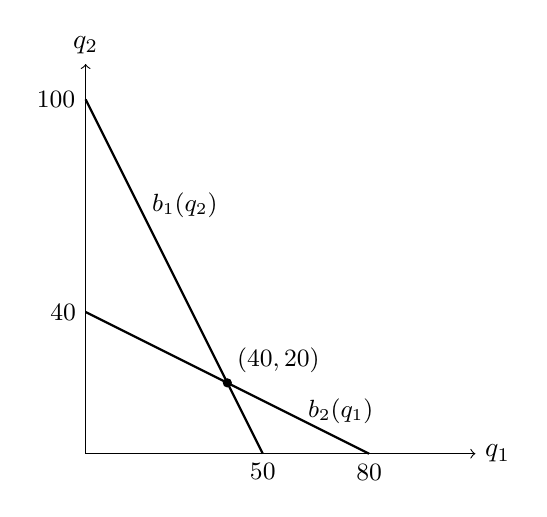
\begin{tikzpicture}[scale=0.045]
\draw[->] (0,0)--(110,0) node[right]{$q_1$};
\draw[->] (0,0)--(0,110) node[above]{$q_2$};
\draw[thick] (50,0)--(0,100) node[left]{\small 100};
\node[below] at (50,0){\small 50};
\node at (28,70){\small $b_1(q_2)$};
\draw[thick] (0,40)--(80,0) node[below]{\small 80};
\node[left] at (0,40){\small 40};
\node at (72,12){\small $b_2(q_1)$};
\fill (40,20) circle (1.3);
\node[above right] at (40,20){\small $(40,20)$};
\end{tikzpicture}
\end{center}
\end{solution}
\item[4.3] Find the Cournot Nash equilibrium $(q_1^c,q_2^c)$, $Q^c$ and $p^c$. Which firm produces more, and why?
\begin{solution}
Here symmetry \emph{cannot} be imposed, so solve the two best responses together. Substitute: $q_1=\frac{100-\frac{80-q_1}{2}}{2}=\frac{120+q_1}{4}\Rightarrow3q_1=120\Rightarrow q_1^c=40$, $q_2^c=(80-40)/2=20$. Then $Q^c=60$ and $p^c=60$.

The low-cost firm produces more. Its marginal cost is lower, so its best response is shifted out.
\end{solution}
\item[4.4] Find each firm's profit, CS, PS and TS.
\begin{solution}
$\pi_1=(60-20)(40)=1600$, $\pi_2=(60-40)(20)=400$. $PS=2000$. $CS=\tfrac12(60)(120-60)=1800$. $TS=3800$.
\end{solution}
\item[4.5] Find the efficient outcome: how much should be produced and \emph{by which firm}? Compute the DWL and decompose it into (i) loss from underproduction and (ii) loss from the wrong firm producing. Illustrate on the $p$--$Q$ plane.
\begin{solution}
Efficiency means producing every unit at the lowest possible cost, so firm 1 ($MC=20$) should produce everything. With $p=20$, $Q^*=100$ and $TS^*=\tfrac12(100)(120-20)=5000$.
\[DWL=5000-3800=1200.\]
(i) Underproduction: the triangle between demand and $MC_1=20$ from $Q=60$ to $100$, $\tfrac12(40)(60-20)=800$.
(ii) Wrong firm: firm 2's $20$ units cost $40$ each instead of $20$, which wastes $(40-20)(20)=400$.
Check: $800+400=1200$.
\begin{center}
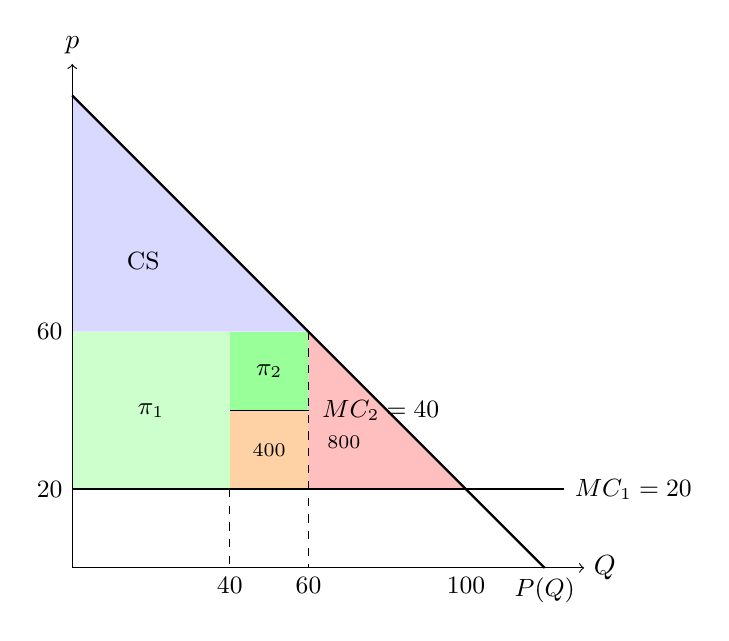
\begin{tikzpicture}[scale=0.05]
\fill[blue!15] (0,120)--(0,60)--(60,60)--cycle;
\fill[green!20] (0,20) rectangle (40,60);
\fill[green!40] (40,40) rectangle (60,60);
\fill[orange!35] (40,20) rectangle (60,40);
\fill[red!25] (60,60)--(60,20)--(100,20)--cycle;
\draw[->] (0,0)--(130,0) node[right]{$Q$};
\draw[->] (0,0)--(0,128) node[above]{$p$};
\draw[thick] (0,120)--(120,0) node[below]{\small $P(Q)$};
\draw[thick] (0,20)--(125,20) node[right]{\small $MC_1=20$};
\draw (40,40)--(60,40);
\node[right] at (61,40){\small $MC_2=40$};
\draw[dashed] (40,20)--(40,0); \draw[dashed] (60,60)--(60,0);
\node[left] at (0,60){\small 60};
\node[left] at (0,20){\small 20};
\node[below] at (40,0){\small 40};
\node[below] at (60,0){\small 60};
\node[below] at (100,0){\small 100};
\node at (18,78){\small CS};
\node at (20,40){\small $\pi_1$};
\node at (50,50){\small $\pi_2$};
\node at (50,30){\scriptsize 400};
\node at (69,32){\scriptsize 800};
\end{tikzpicture}
\end{center}
The orange rectangle is the wrong-firm loss and the red triangle is the underproduction loss.
\end{solution}
\item[4.6] Suppose firm 1's marginal cost falls from $20$ to $14$. Find the new equilibrium and explain how each firm's quantity and the price respond.
\begin{solution}
In general, $q_1^c=(A-2c_1+c_2)/3$ and $q_2^c=(A-2c_2+c_1)/3$. With $c_1=14$: $q_1^c=(120-28+40)/3=44$, $q_2^c=(120-80+14)/3=18$, $Q^c=62$, $p^c=58$.

Each \$1 fall in $c_1$ raises $q_1$ by $2/3$, lowers $q_2$ by $1/3$ (strategic substitutes: firm 2 contracts when firm 1 expands), raises $Q$ by $1/3$ and lowers $p$ by $1/3$.
\end{solution}
\item[4.7] For what values of $c_2$ (holding $c_1=20$) does firm 2 produce a positive quantity in equilibrium? What happens otherwise?
\begin{solution}
$q_2^c=(120-2c_2+20)/3>0\iff c_2<70$. If $c_2\ge70$, firm 2's best response to firm 1 is $0$ (truncate at zero), and firm 1 acts as a monopolist: $q_1=(120-20)/2=50$, $p=70$. Firm 2 then cannot profitably enter, since $p=70\le c_2$.
\end{solution}
\end{description}
\end{document}
